%%%%%%%%%%%%%%%%%%%%%%%%%%%%%%%%%%%%%%START PREAMBLE THAT IS THE SAME FOR ALL EXAMPLES
\documentclass{article}

%Required: You must have these
\usepackage{Sweave}
\usepackage{graphicx}
\usepackage{tabularx}
\usepackage{hyperref}
\usepackage{natbib}
\usepackage{pdflscape}
\usepackage{array}
\usepackage{authblk}
\usepackage{gensymb}


%\usepackage[backend=bibtex]{biblatex}
%Strongly recommended
 %put your figures in one place
%\SweaveOpts{prefix.string=figures/, eps=FALSE} 
%you'll want these for pretty captioning
\usepackage[small]{caption}

\setkeys{Gin}{width=0.8\textwidth} %make the figs 50 perc textwidth
\setlength{\captionmargin}{30pt}
\setlength{\abovecaptionskip}{10pt}
\setlength{\belowcaptionskip}{10pt}
% manual for caption http://www.dd.chalmers.se/latex/Docs/PDF/caption.pdf

%Optional: I like to muck with my margins and spacing in ways that LaTeX frowns on
%Here's how to do that
\topmargin -1.5cm    
\oddsidemargin -0.04cm  
\evensidemargin -0.04cm % same as oddsidemargin but for left-hand pages
\textwidth 16.59cm
\textheight 21.94cm 
%\pagestyle{empty}    % Uncomment if don't want page numbers
\parskip 7.2pt      % sets spacing between paragraphs
%\renewcommand{\baselinestretch}{1.5} 	% Uncomment for 1.5 spacing between lines
\parindent 0pt% sets leading space for paragraphs
\usepackage{setspace}
%\doublespacing
\renewcommand{\baselinestretch}{1.8}
\usepackage{lineno}
%Optional: I like fancy headers
%\usepackage{fancyhdr}
%\pagestyle{fancy}
%\fancyhead[LO]{How do climate change experiments actually change climate}
%\fancyhead[RO]{2016}
 
%%%%%%%%%%%%%%%%%%%%%%%%%%%%%%%%%%%%%%END PREAMBLE THAT IS THE SAME FOR ALL EXAMPLES

%Start of the document
\begin{document}

%\SweaveOpts{concordance=FALSE}
\Sconcordance{concordance:sm_doc.tex:sm_doc.Rnw:%
1 223 1}


\bibliographystyle{../../Bibliography/bibstyles/amnat.bst}
\title{Soil moisture interacts with temperature to affect plant phenology} %
\author[1,2,a]{A.K. Ettinger}
\author[3,b]{J.S. Dukes}
\author[4,c]{M.R. Johnston}
\author[5,d]{C.R. Rollinson}
\author[1,4,6,e]{E.M. Wolkovich}

\affil[1]{Arnold Arboretum of Harvard University, Boston, Massachusetts 02131, USA}

\affil[2]{The Nature Conservancy,Seattle, Washington, USA}


\affil[3]{Department of Forestry \& Natural Resources and Department of Biological Sciences, Purdue University, West Lafayette, Indiana 47907, USA}

\affil[4]{Department of Organismic \& Evolutionary Biology, Harvard University, Cambridge, Massachusetts 02138, USA}

\affil[5]{The Morton Arboretum, Lisle, Illinois 60532, USA}

\affil[6]{Forest \& Conservation Sciences, Faculty of Forestry, University of British Columbia, Vancouver, BC, Canada}

\affil[a]{Corresponding author; email: ailene.ettinger@tnc.org; phone: 781-296-4821; mailing address: 73 Wall Street. Seattle, WA 98121, USA }

\date{\today}
\maketitle %put the fancy title on
%\tableofcontents %add a table of contents
\textbf{Author contributions}: All authors conceived of this manuscript, which began at a Radcliffe Exploratory Seminar in 2016, and all authors contributed to manuscript revisions. AKE and EMW conceived of the idea for the literature review, database compilation, and related Radcliffe Exploratory Seminar. AKE compiled the datasets; AKE analyzed the data and created the figures.

\textbf{Data Accessibility} 
The data reported in this paper are from the MC3E and ExPhen databases, which are available at KNB \citep{ettinger2018,ettinger2021}

\textbf{Running title} Soil moisture affects phenology

\textbf{Key words} global warming, warming experiment, microclimate, phenology, bud-burst, leaf-out, flowering, fruiting, senescence 


\textbf{Paper type} New Phytologist
%Brief Communications-Brief Communications are short (c 3000-4000 word) research articles reporting exciting, significant new findings. They include no more than 4 figures and tables, combined. Manuscripts, and their abstracts, should be organized as described for Research articles. Authors must adhere to the same membership and page charge requirements as for regular Research Articles.
%\textbf{Number of words in abstract} 

%\textbf{Number of words in main text} 

%\textbf{Number of references} 

%\textbf{Number of tables} 0

%\textbf{Number of figures} 


%%%%%%%%%%%%%%%%%%%%%%%%%%%%%%%%%%%%%%%%%%%%%%%%%%%

%%%%%%%%%%%%%%%%%%%%%%%%%%%%%%%%%%%%%%%%%%%%%%%%%%%
\linenumbers
\section*{Abstract}
Previous meta-analyses of phenology responses to climate change have focused largely on temperature as a driver of observed shifts. However, soil moisture is also affected by climate change and likely to alter biological responses. Here we synthesize microclimate and phenology data from climate change experiments to quantify how soil moisture interacts with temperature to affect plant phenology. We find that soil drying generally delays plant phenology, especially for budburst, for which this delay occurs at a rate of 0.42 days per percent reduction in soil VWC. The magnitude of effects we quantify suggest that climate change-induced shifts in soil moisture will generally play a small role in altering future phenology, compared to shifts in temperature, both because of the strong sensitivity of plant phenology to temperature and because of the large magnitude of projected shifts in temperature, compared to shifts in soil moisture. Nonetheless, although effects of soil moisture are comparably small across all species in our analysis, sensitivity to soil moisture varied dramatically by species, and soil moisture levels differed by site and among years. Thus, soil moisture is likely to play a role in phenological shifts with climate change for some species, in some locations and years. Quantifying phenological sensitivity to changes in soil moisture will therefore likely improve forecasts of shifts in phenology with future climate change at the fine spatial scales relevant for management and conservation.  

\newpage
\section* {INTRODUCTION}
\par Climate change is affecting organisms by altering temperature and soil moisture around the world \citep{parmesan2006,chen2011}. One of most widespread biological responses to climate change is a shift in phenology, the timing of recurring biological events, which has occurred at a rate of 2.3-5.1 days per decade \citep{parmesan2006,poloczanska2013,root2003}. Shifts in plant phenology are the most widely documented, with spring phenology (budburst, leaf-out, and flowering) occurring earlier in recent years \citep{wolkovich2012}, and senescence occurring later \citep{taylor2008,delpierre2009}. 
\par Phenological shifts are typically attributed to warming temperature, a known and well-studied driver of plant phenology. The timing of spring budburst, for example, depends on temperature through both chilling (the prolonged exposure to cold temperatures after growth cessation in the fall) and forcing (exposure to warm temperatures). (introduce GDD, if that part is kept in the paragraph and if we include GDD models) Recent trends of advancing phenology may be due to increases in both/either chilling and/or forcing with global warming \citep{fujisawa2010, ibanez2010,cook2012b}. In places where delays in spring phenology have occurred, reductions in winter chilling are often the attributed cause \citep{yu2010}. 
\par Effects of altered precipitation and soil moisture on phenology have received less attention, but are likely to be important drivers of plant phenology. For example, budburst, flowering, and leaf drop are affected by tree water status in dry ecosystems \citep[e.g., ][]{essiamah1986,reich1984, van1993}. Budburst can be slowed by water stress through inhibiting cell elongation \citep{essiamah1986}, and growing season start may be delayed by drought in grasslands \cite{cui2017}. Flowering phenology, on the other hand, can be advanced by drought conditions \citep{hamann2018}. When effects of soil moisture on phenology have been quantified, this has occurred largely in arid and grassland or meadow ecosystems (e.g., Cleverly 2016, Tao et al 2019, Ganjurjac et al 2020); its role in other ecosystem types is less explored.
\par could add a paragraph on challenges ofobservational studies of soil moisture vs temperature as drivers because they are often correlated/affect one another? Or something about interactions between temperature and moisture? 
\par Here we conduct a meta-analyses of climate change experiments to test whether and how soil moisture interacts with temperature to affect plant phenology. Field-based climate change experiments that warm plots to different levels offer valuable tools to study climate change impacts on plant phenology. Experiments can combine temperature and precipitation treatments to create the ``no-analog" climate scenarios forecasted for the future, particularly when they employ active-warming methods, such as forced air heaters, soil warming cables, or infrared heaters \citep{shaver2000,williams2007b,aronson2009}. Climate change experiments often monitor daily soil moisture, as well as daily air temperature, at the plot-level, allowing detailed quantification of how microclimate affects plant phenology. 
\par Previous meta-analyses of phenology in climate change experiments have focused primarily on effects of temperature \citep[e.g.,][]{wolkovich2012}. We expected that soil moisture may also affect phenology, with drier soils delaying budburst and leafout phenology and advancing flowering and fruiting phenology). We wanted to test interactive effects of soil moisture and temperature on phenology, as well as how shifts in soil moisture affect the cumulative growing degrees at which a phenological event occurs.   We use measured microclimate and phenology data from two databases of climate change experiments: MicroClimate from Climate Change Experiments \citep[MC3E, ][]{ettinger2018}) and Experimental Phenology (ExPhen)  to quantify effects of soil moisture and above-ground temperature on plant phenology (bud-burst, leaf-out, flowering, fruiting, senescence; see Materials and Methods). We also use forecasted changes in temperature and soil moisture to investigate how including soil moisture alters expected future shifts in phenology. 
%Do we want to spell out any of the following specific quesitons suggested by Lizzie here?
%1) Are the temp and moisture effects synergistic or mainly acting alone? (I think lots of ecologists -- myself included -- think there will or should be a big interaction so we should test it explicitly. If we don't see one, that's interesting.)
%2) How consistent are the effects across sites, phenophases, life forms and species? (I don't think we want to answer all of these a priori based on the data, but it might help readers if we clarify what we do and do NOT plan to try to compare.)
%3) Under what circumstances will forecasting moisture effects on plant phenology matter the most? (I think our answer for now is that it's mainly about some species -- Figure 3? I like this answer, we may just want to back it up some and think if we can use the posteriors better to put some numbers on species-level variance versus site or such?) [Are species nested within site? Also, should we plot the mu values as one panel in Fig 3 so then it would be a four figure panel? Not sure if this possible, I often dream up stuff that we can't get out of models, but wanted to suggest it in case.]


\section* {MATERIALS AND METHODS}
\textbf {\emph{Data}}-- To investigate how soil moisture interacts with temperature to affect phenology, we used two databases that compiled data from climate change experiments. Microclimate data came from the  MicroClimate from Climate Change Experiments (MC3E) database \citep{ettinger2018}. Phenology data came from a ExPhen, a new database of phenology from climate change experiments \citep{ettinger2021}. 
\par Both databases were created by first identifying published, active-warming field experiments, many of which included precipitation manipulations. We focused on \textit{in situ} active-warming manipulations because recent analyses indicate that active-warming methods are the most controlled and consistent methods available for experimental warming \citep{kimball2005,kimball2008,aronson2009,wolkovich2012}. We carried out a full literature review to identify potential active-warming field experiments, following the methods and search terms of \citet{wolkovich2012} for their Synthesis of Timings Observed in iNcrease Experiments (STONE) database \citep{wolkovich2012}, but restricting our focus to active-warming experiments. Further, because our goal was to tease out variation in microclimate (including temperature and soil moisture), we focused on warming studies that included both/either multiple levels of warming and/or precipitation treatments. These additional restrictions constrained the list to 11 new studies published after the STONE database, as well as six of the 37 studies in the STONE database. We contacted authors to obtain daily microclimate and phenological data for these 17 studies and received data (or obtained publicly available data) for 10 of them, as well as datasets from five additional sites offered or suggested to us over the course of our literature review and data analysis. The daily temperature and soil moisture data from these 15 experiments comprise the MC3E database, which is available at KNB \citep{ettinger2018}. The phenology data from these 15 experiments comprise the ExPhen database of experimental phenology, which is also available at KNB \citep{ettinger2021}.

\textbf {\emph{Analysis}}--
To understand how soil moisture interacts with temperature to affect phenology, we fit models with microclimate predictor variables of measured soil moisture, measured temperature, and their interaction to phenology response data (budburst, leafout, flowering, fruiting, senescence). Microclimate data came from the MC3E database, and phenology data came from the ExPhen database. We excluded conifers from the analysis, because their phenology has distinct differences from angiosperm phenology \cite{polgar2014} and conifer data existed from only one site in the database. For all phenophases, the response variable was day-of-year of the phenological event. Predictors for our primary models were measured air temperature, soil moisture, and their interaction. Random effects for all phenology models were species (with random slopes and intercepts), site (random intercept), and year nested within site (random intercept). Equations for these models can be found in the Supplemental Methods. 

\par To better understand how shifts in soil moisture may alter phenology under climate change, we additionally fit phenology models in which the response variable was cumulative growing degree dats at the time of the phenological event and the predictor variable was measured soil moisture.  
%\par To quantify how climate manipulations affect temperature an
%\par \underline{Keep or cut the below, or move to supp?} 
%\par To better understand the interactive effects of measured temperature and soil moisture, experimental treatment effects, and feedbacks between temperature and soil moisture conditions, we conducted follow-up analyses in which we fit the same phenology models to subsets of the data (controls only, low temperature treatments only, and high temperature treatments only). We also fit a model with soil temperature in place of air temperature, for the subset of sites these data were available. 
%\par To quantify how climate manipulations affect temperature and soil moisture, we used microclimate data from the 4 sites in the MC3E database that manipulated both precipitation and temperature, and measured both above-ground temperature and soil moisture (exp01,exp05,exp07,exp12). We then fit two groups of hierarchical models to microclimate data from these sites: one group with temperature response variables (including mean annual, and mean seasonal temperatures), and the other group with soil moisture as response variables (including mean annual, and mean seasonal soil moisture). For both groups of models, explanatory variables were temperature treatment, precipitation treatment, and their interaction. The models included a random effect of site, with a random slope and intercept structure, to allow effects of experimental treatments to vary across sites. Models also included random effects of day-of-year, nested within year, on the intercept only, to account for non-independence of measurements taken on the same day within the same year. Equations for these models can be found in the Supplemental Methods. 

\section* {RESULTS}

We found that soil drying delays phenology and warming temperatures advance phenology, for most phenophases. The magnitude of these effects varies across phenophases, species, and sites. Add sumamry sentence about life forms (trees, shrubs, herbs, grasses, Fig \ref{fig:forms})? And ecosystems, if we add grassland vs forest comparison.
\par Effects of soil moisture were strongest for budburst and leafout, and affected all phenophases except fruiting (Figures \ref{fig:bblo}, 1S). Soil drying delays spring budburst at a rate of 0.42 days per percent reduction in soil VWC. Thus, if soil moisture is reduced by 10\% of its current state (mean across all sites for which budburst was monitored= XX), as is expected over the next 50 years in the northeastern US \citep{berg2017} budburst would be delayed by approximately XX days on average, due to changes in soil moisture alone.

\par  Increasing air temperature advanced phenology for all phenophases except senescence (Figure 1S). Our models estimate that warming advances budburst phenology at a rate of 3.42 days per \degree C, advances leafout at a rate of XX, advances flowering a rate of XX, and advances fruiting at a rate of XX These estimates are consistent with estimates from previous meta-analyses \citep{wolkovich2012}. 

\par  Add a paragraph about GDD models

%\par \underline{Keep or cut the below, or move to supp?}% Lizzie says to reference and include the as many different analyses as possible 
%\begin{itemize}

%\item \textbf{Soil moisture effect size is bigger in full dataset than in controls only, for BB.} Mean and range of SM is similar (though max is a bit higher in full dataset; min is similar).
%\item \textbf{Effects of climate manipulations on temperature and soil moisture}
%\end{itemize}
%\par Mean annual soil moisture is negatively affected by target temperature treatment, and positively affected by precipitation treatment. (Figure \ref {fig:soilmois}). These effects varied by site; for example, at exp07 soil moisture was positively affected by temperature treatment. Air temperature is positively affected by target temperature treatment, and negatively affected by precipitation treatment. (Figure S\ref {fig:temp}).

\section* {DISCUSSION}
\par  Across the life forms included in the ExPhen database (Table \ref{tab:studylocs}), soil moisture affects phenology. Soil moisture had previously been investigated primarily in arid ecosystems (e.g. XXX), and has not been a focus of experiments and meta-analyses (e.g. Wolkovich). We quantify effects of soil moisture across forest and grassland ecosystems.

\par Effects of temperature and soil moisture, and their interaction, on phenology vary across phenophases and species .
- Discussion of functional groups- trees, shrubs, grasses, forbs.

 \par Global change factors interact to affect phenology.  
 -temperature and soil moisture here
 -also interactions with CO2
 -limiting resources: Variable responses to moisture (and precip) may be caused by temporal and spatial variation in the most limiting resource (e.g., temperature vs moisture). As global warming reduces temperature limitation, importance of moisture limitation in plant phenology may increase. 

\par Relating experiements to "real world:
    -Moving beyond treatments levels to analyze plot-level microclimate- closer to how plants may be experiencing treatments
    -how temperature is affected by soil moisture, and how soil moisture is affected by temperature treatments

\par What is per unit effect of soil moisture change on different phenophases? (We do say this one already and it seems mostly done?)
\par What is the effect of soil moisture change relative to temperature on different phenophases? That is, can we compare them given a 10\% increase in mean temperature or a 1 SD change? (Lizzie think this would be cool if we can think of a good way to do it ... 
\par Are the temp and moisture effects synergistic or mainly acting alone? (Lizzie thinks lots of ecologists -- herself included -- think there will or should be a big interaction so we should test it explicitly. If we don't see one, that's interesting.)
\par How consistent are the effects across sites, phenophases, life forms and species? (I don't think we want to answer all of these a priori based on the data, but might want to spell ou what we do want to compare)
\par Under what circumstances will forecasting moisture effects on plant phenology matter the most? (I think our answer for now is that it's mainly about some species -- Figure 3? I like this answer, we may just want to back it up some and think if we can use the posteriors better to put some numbers on species-level variance versus site or such?) [Are species nested within site? Also, should we plot the mu values as one panel in Fig 3 so then it would be a four figure panel? Not sure if this possible, I often dream up stuff that we can't get out of models, but wanted to suggest it in case.]


\section* {Conclusions}

\section* {Questions for Lizzie at this stage}

2) What other figures do you think would strengthen/support the paper?

3) Target Journal: New Phytologist? Or somewhere else?


\bibliography{../../Bibliography/mylibrary.bib}

\section*{Figures}

\begin{figure}[h]
\centering
 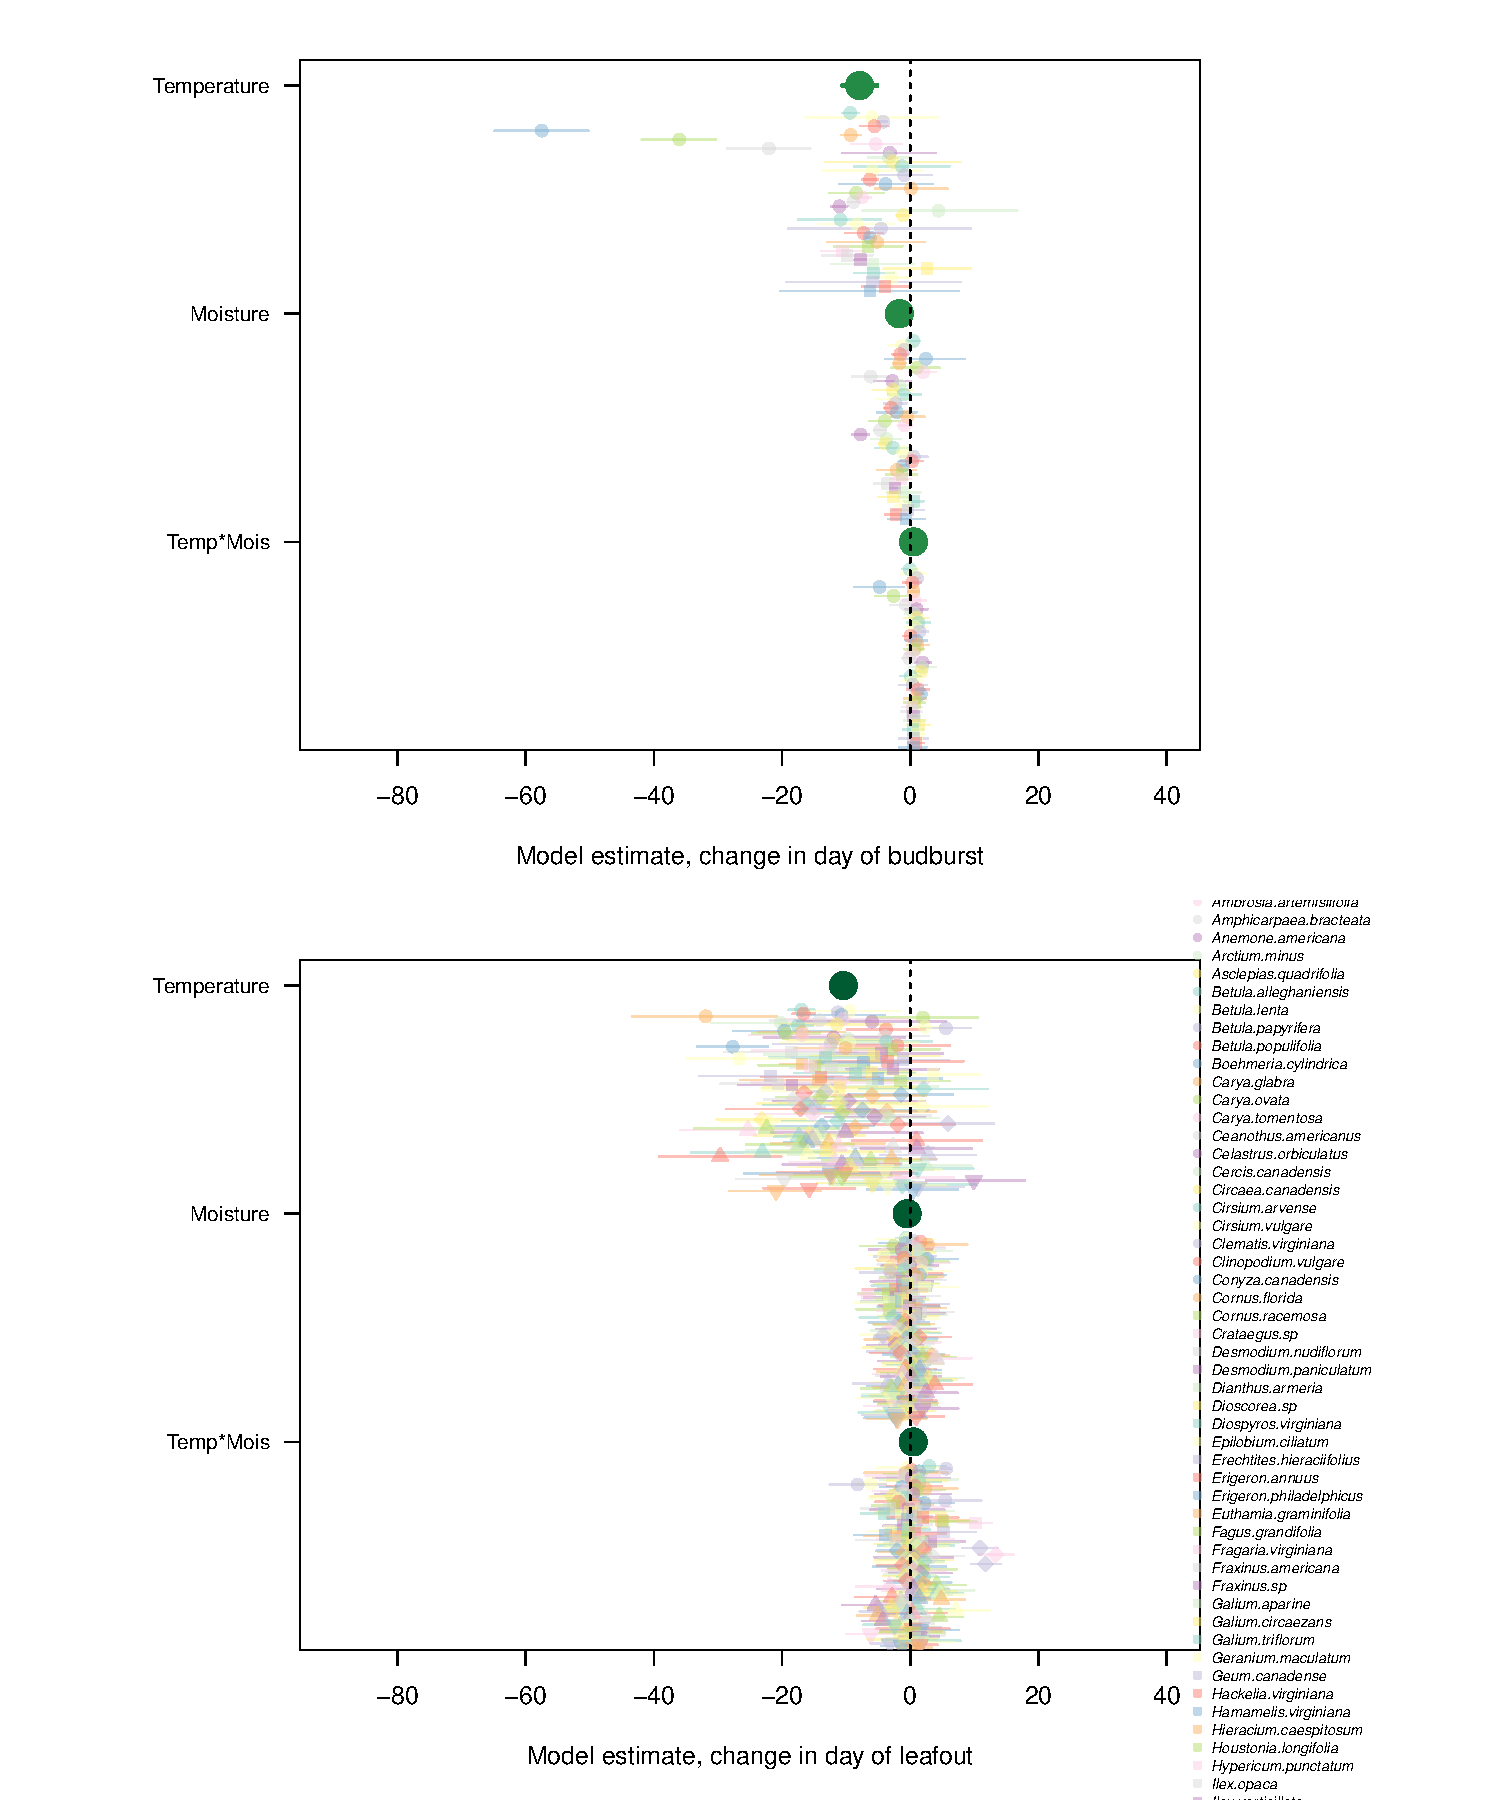
\includegraphics{../../Analyses/soilmoisture/figures/m5_bbdlo_.pdf}
 \caption{\textbf{Model coefficients from budburst and leafout models (with centered predictors).}} 
 \label{fig:bblo}
 \end{figure}
 
\begin{figure}[h]
\centering
 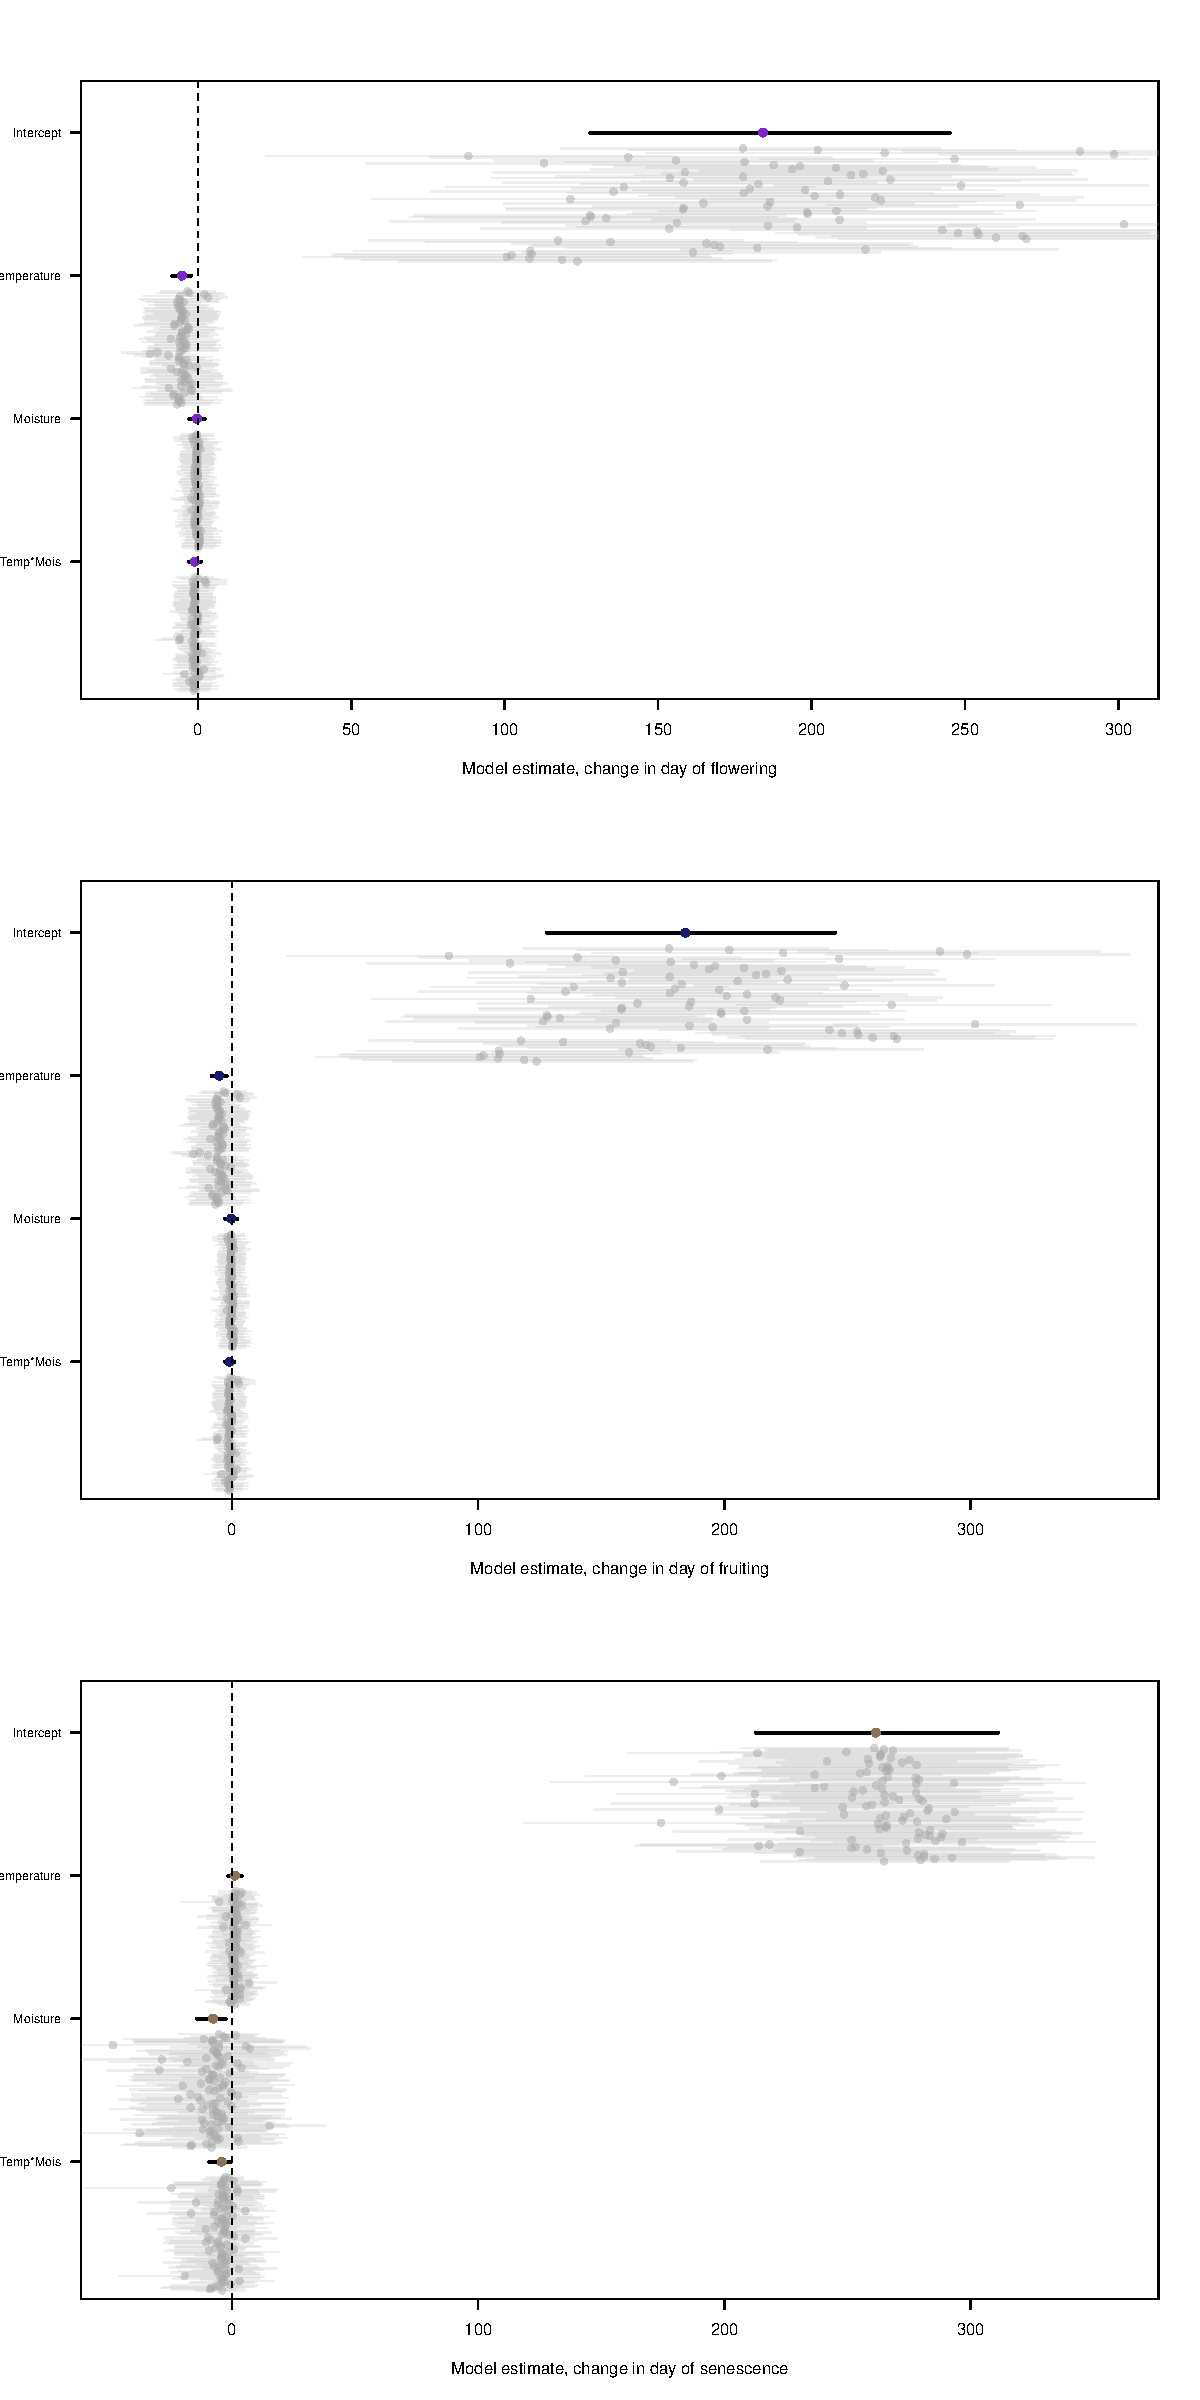
\includegraphics[width=0.65\textwidth]{../../Analyses/soilmoisture/figures/m5_ffd_frd_sen.pdf}
 \caption{\textbf{Model coefficients from flowering, fruiting, and senescence models (with centered predictors). Move to Supp! Also, remove intercept.}} 
 \label{fig:flfr}
 \end{figure}
 
 
 \begin{figure}[h]
\centering
 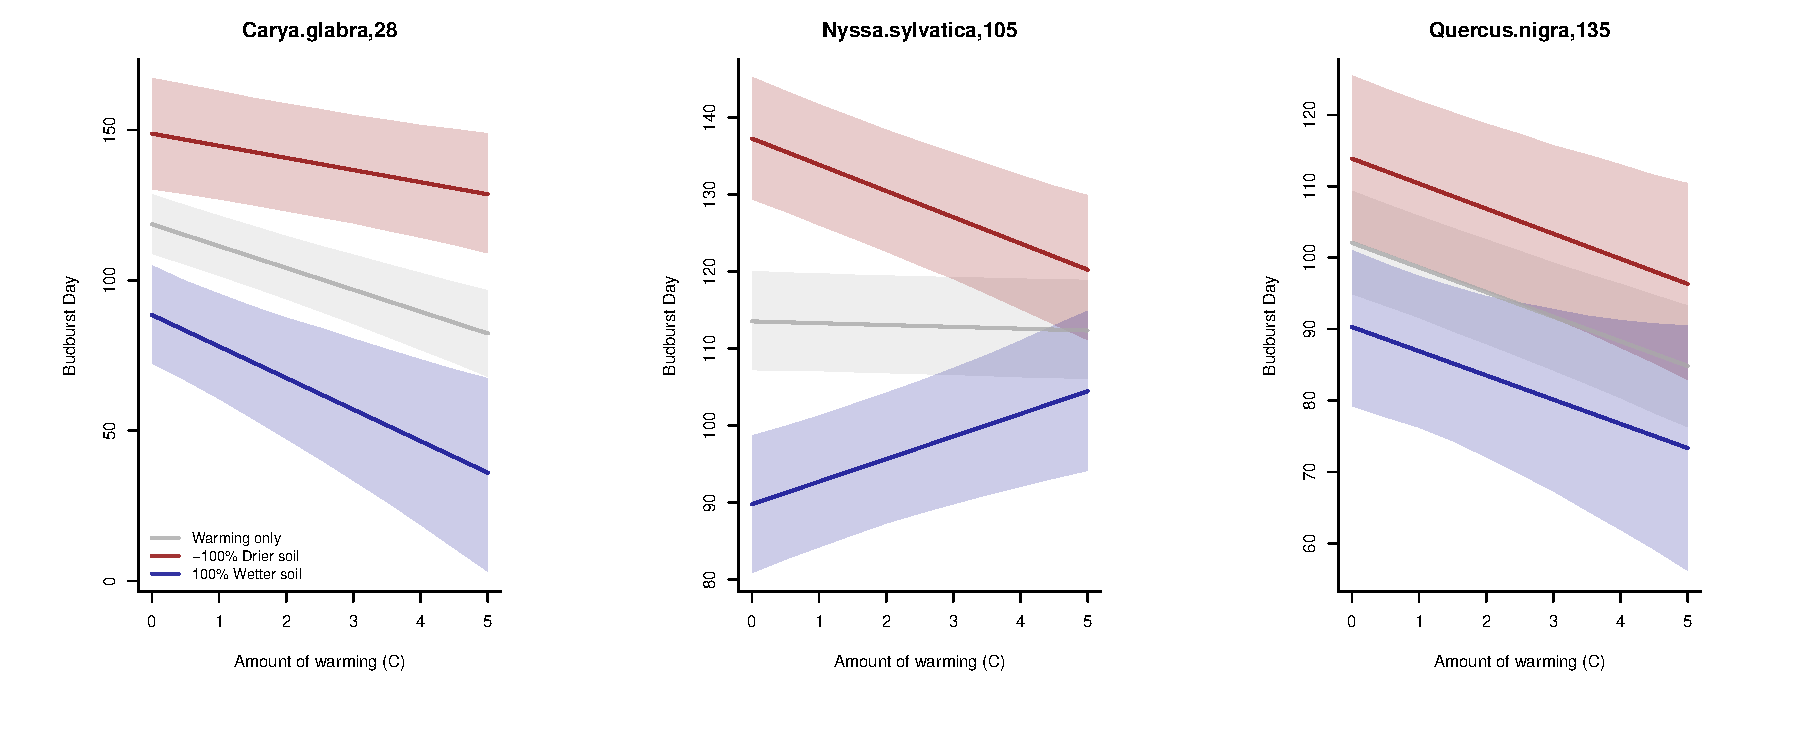
\includegraphics{../../Analyses/soilmoisture/figures/tempforecast_bb_0_5_28_105_135_NA_4_degwarm.pdf}
 \caption{\textbf{Patterns of forecasted changes in budburst date with warming and shifts in soil moisture vary across species}. For nearly all species, our model estimated negative effects (i.e., earlier) of both temperature and soil moisture on budburst; however, the magnitude of these effects, as well as the sign and magnitude of the estimated interaction between soil moisture and temperature, differed across species, potentially resulting in divergent patterns with forecasting changes in climate change.  Budburst may occur much earlier in wetter vs drier soils with warming for species such as \textit{Carya glabra} (left panel), with a strong estimated negative interaction between soil moisture and temperature. Other species, such as \textit{Nyssa sylvatica}(middle panel), may experience delayed budburst in wet soils but advances in dry soils, with a strong positive interaction between moisture and temp. Still other species' budburst, such as \textit{Quercus nigra} (right panel), exhibits weak interactive effects of temperature and soil moisture and are therefore likely to advance with warming regardless of changes in soil moisture.}
 \label{fig:bbsp}
 \end{figure}
 
  
 \begin{figure}[h]
\centering
 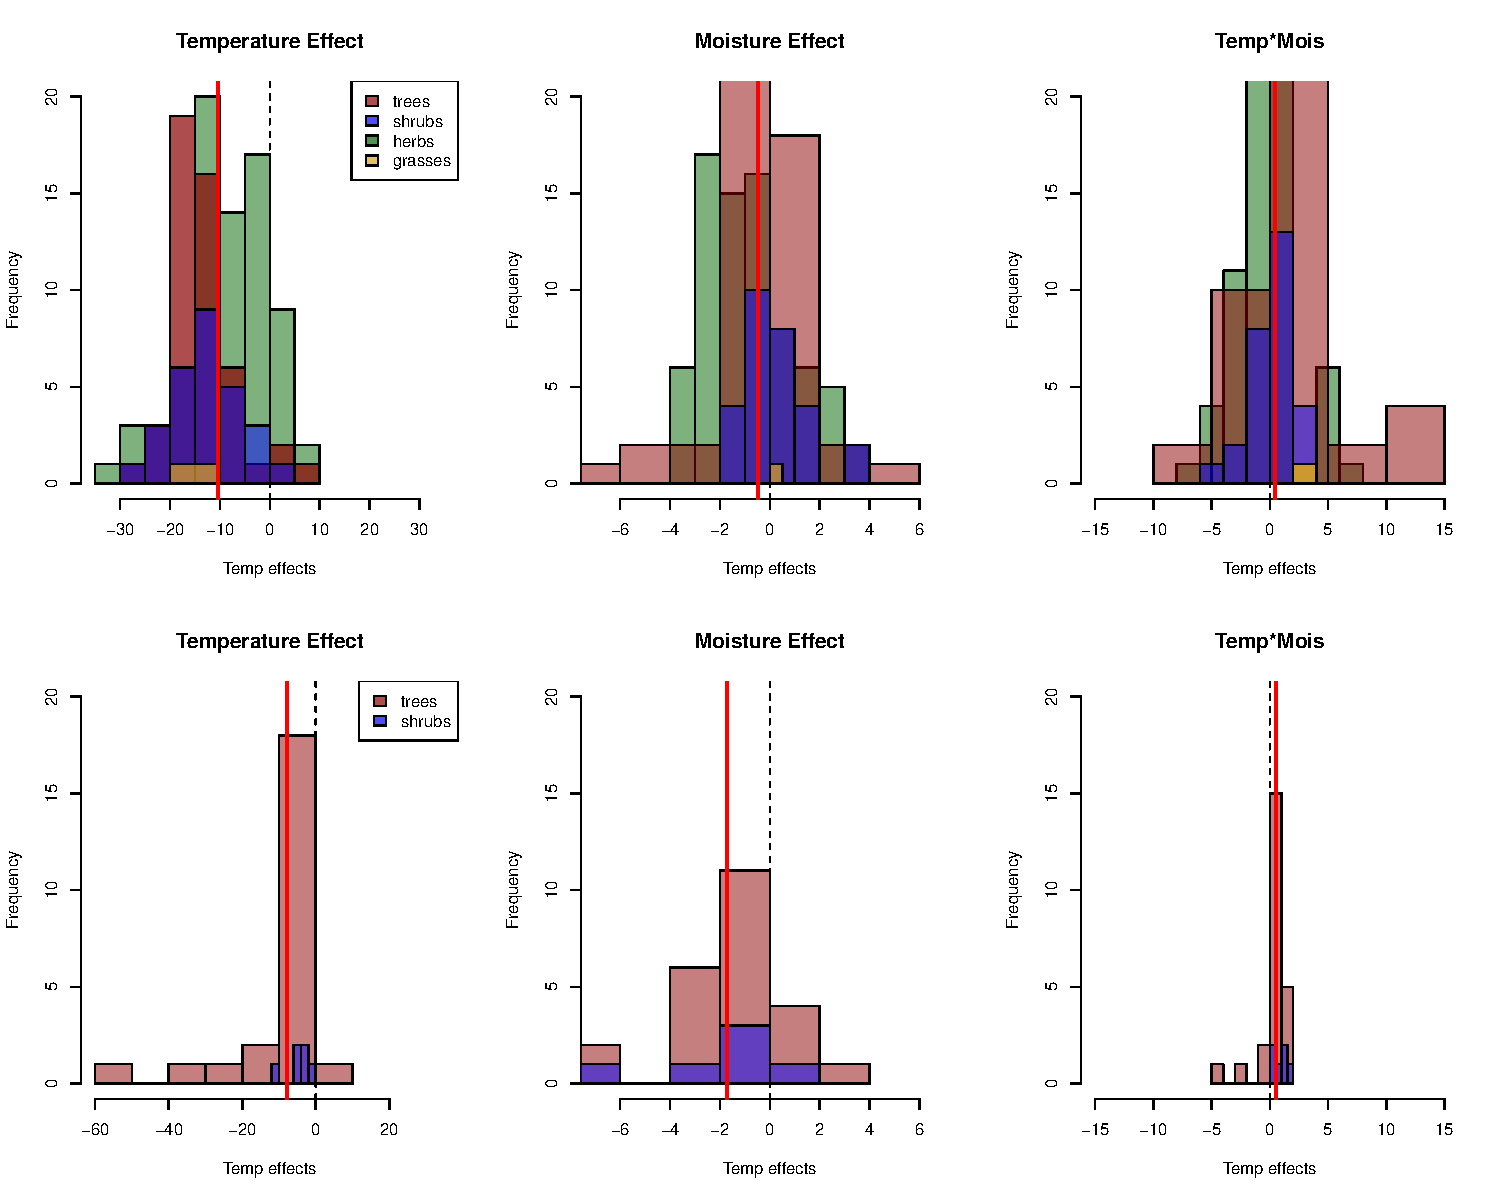
\includegraphics{../../Analyses/soilmoisture/figures/histbbloform_spef.pdf}
 \caption{\textbf{Effects of temperature, soil moisture, and their interaction do not differ strongly across life forms}.}
 \label{fig:forms}
 \end{figure}
 

 \par Additional Figures to make:
 \begin{itemize}
 \item Plots of (mean?) soil moisture and temperature by site, year, and phenophase
\item Histograms by form and/or ecosystem
 \item Map of studies with symbols varying by ecosystem? (for Supp)
\item Tables of models (for Supp)
\end{itemize}

 %2. Reach out to Christy, Miriam and Jeff when the figures are done and be clear that  Make it clear that this is pretty finished. 
 
 
%%%%%%%%%%%%%%%%%%%%%%%%%%%%%%%%%%%%%%%%
\end{document}
%%%%%%%%%%%%%%%%%%%%%%%%%%%%%%%%%%%%%%%%
